%\documentclass[10pt,oneside,letterpaper,twocolumn]{article}
\documentclass[sigconf]{acmart}
%\usepackage[a4paper, total={6in, 8in}]{geometry}
\usepackage{times}
\usepackage{verbatim}
\usepackage{outlines} % For outlines
\usepackage{multirow}
\usepackage{enumitem} 
\usepackage{algorithm}
\usepackage{algpseudocode}
\usepackage{graphics,color,url}
%\usepackage[colorlinks=true, allcolors=blue]{hyperref}
\usepackage{array}

\usepackage{amsmath,amsthm, amssymb,eufrak}
\usepackage{enumitem}
\usepackage{float}

% For outlines
\setenumerate[1]{label=\Roman*.}
\setenumerate[2]{label=\Alph*.}
\setenumerate[3]{label=\roman*.}
\setenumerate[4]{label=\alph*.}

\newcommand{\jim}[1]{{{\color{blue} \textbf{Jim: #1}}}}

\newcommand{\commentout}[1]{}

\newtheorem{thm}{Theorem}[section]
\newtheorem{defn}{Definition}[section]

\DeclareMathOperator{\sign}{sgn}
\DeclareMathOperator*{\argmin}{arg\,min}
\newcommand{\real}{\mathbb{R}}
\newcommand{\vect}[1]{\mathbf{#1}}
\newcommand{\vx}{\vect{x}}


\newcommand{\solverset}{\mathcal{S}}
\newcommand{\solver}{s}
\newcommand{\param}{p}
\newcommand{\paramset}{P}
\newcommand{\config}{c}
\newcommand{\bestobj}{\rho}
\newcommand{\exectime}{T}



\newcommand{\transfunc}{\Gamma}
\newcommand{\behaviorfunc}{\Phi}
\newcommand{\outsig}{y}

\newcommand{\initcond}{X_0}
\newcommand{\paramsorig}{v}
\newcommand{\inputs}{u}

\newcommand{\outsigset}{\mathcal{Y}}
\newcommand{\outspace}{Y}
\newcommand{\inputsigset}{\mathcal{U}}
\newcommand{\inputspace}{U}
\newcommand{\timeinterval}{\mathcal{I}}
\newcommand{\inputparams}{\hat{u}}
\newcommand{\inputparamset}{\hat{\mathcal{U}}}
\newcommand{\inputgenerator}{g}

\newcommand{\stateset}{\mathcal{X}}
\newcommand{\paramsorigset}{\mathcal{V}}
\newcommand{\inputset}{\mathcal{U}}



% STL
\newcommand{\F}{\Diamond}
\newcommand{\G}{\Box}
\newcommand{\U}{\mathcal{U}}
\newcommand{\spec}{\varphi}
\newcommand{\true}{\top}
\newcommand{\robparam}{\widehat{\rho}}

\newcommand{\lt}{<}
\newcommand{\rt}{>}


\title{Metaheuristics to falsify properties of cyber-physical systems}

\author{Thao Dang}
\affiliation{%
  \institution{Verimag, France}
}
\email{Thao.Dang@imag.fr}

\author{Alexandre Donz{\'{e}}}
\affiliation{%
  \institution{Decyphir, France}
}
\email{alex@decyphir.com}

\author{James Kapinski}
\affiliation{%
  \institution{Toyota Research Institute - North America}
}
\email{jim.kapinski@toyota.com}

\author{Hisahiro Ito}
\affiliation{%
  \institution{Toyota Research Institute - North America}
}
\email{hisahiro.ito@toyota.com}

\date{}

\begin{document}


\begin{abstract}
Cyber-physical systems (CPSs) are used in many mission-critical applications, and the scale and complexity of these systems is growing rapidly.
New approaches are needed to increase the confidence in the correctness of complex CPS designs.
Falsification techniques offer a practical solution. 
A falsification method takes a system model, along with a specification that defines the correct behavior of the system, and performs a best-effort search over inputs and system parameters for behaviors that violate the specification, essentially performing automated bug finding.
Falsification methods rely on a global optimizer to guide the search; one challenge with falsification is that it can be difficult to select the most effective optimizer and optimization parameters.
To address this, we introduce a new adaptive search strategy that automatically focuses computing resources on the most effective optimizer for a given falsification task.
Given a collection of optimizers, our approach makes heuristic decisions to switch optimizers based on
evolving measures of both cost and the coverage of the decision space.
The technique is able to automatically falsify properties for complex CPS design models more efficiently than existing techniques.
We demonstrate the efficacy of the approach using several examples, including an automotive powertrain control system.
\end{abstract}

\maketitle


\iffalse
\begin{outline}[enumerate]
\1 Introduction
	\2 The challenge of falsification
	\2 Falsification generally and via STL for CPS
	\2 Coverage
	\2 Metaheuristics in optimization
	\2 Overview of our approach
\1 Preliminaries: \emph{For much of the notation, we can reuse the notation from the CAV paper with Arvind, as it provides a way to introduce STL, robustness, and falsification but then quickly move to a general global optimization setting.}
	\2 General notation
		\3 $\Pi$ is a set of global optimization solvers
		\3 For a given solver $\pi\in \Pi$, $\Theta$ is a set of solver \emph{configurations}
		\3 $J$ is a cost evaluation
		\3 $x(t)$ is a trace of the system
	\2 Falsification
	\2 STL
		\3 $\varphi$ is an STL property 
		\3 $\rho$ maps a trace and an STL formula to a real number
	\2 Coverage
		\3 $H$ takes a collection of points and maps it to a real number representing the \emph{coverage} of the space points.
\1 Method
	\2 Monitoring robustness and coverage across iterations
	\2 Changing solver based on heuristic rules, informed by robustness and coverage
	\2 F-Race for tuning parameters
\1 Experiments
\1 Conclusions
\end{outline}
\fi

\section{Introduction} \label{sec:introduction}

Development of hybrid and cyber-physical systems (CPS) is becoming
increasingly challenging as the designs for modern CPS become more and
more complex.  As these systems are found in many safety-critical
applications, like aircraft, medical devices, and automobiles, it is
vital that they behave in a manner consistent with their
design expectations. Despite this, it is difficult to verify that CPS
designs meet their requirements for complex applications.

Property \emph{falsification} has garnered much interest recently as a
way to perform automatic bug-finding for complex CPS design
models. Falsification can be thought of as testing where requirements
are expressed in a formal specification language such as temporal
logic.  Two such languages that are appropriate for CPS applications
are metric temporal logic (MTL) and signal temporal logic (STL)
\cite{Koymans1990,MalerN04} for specifying behaviors defined using
real-valued signals over dense time. A key feature of MTL and STL is
that they are equipped with \emph{robust} semantics, and for a given
behavior, methods exist to efficiently compute a real value, called
the robustness which quantifies the requirement satisfaction level of
the behavior \cite{FainekosP06fates,DonzeM10}. A positive robustness
value indicates the behavior satisfies the requirement; a negative
robustness value indicates the behavior does not satisfy the
requirement. Falsification procedures use the robustness as the
objective function for a global optimizer, which seeks a behavior with
negative robustness value. Thus, the optimizer can be used to
automatically find behaviors that violate (falsify) the
requirement. Falsification techniques have been applied to many CPS
systems and are finding application in industry, using tools like
S-TaLiRo and Breach \cite{TaliroLFS11,BreachCAV10}.

This CPS falsification approach is faced with the following majors
challenges.  First, this approach often requires optimization over
continuous-time input signal spaces, whereas existing optimization
solvers expect a finite-dimensional of decision variables.  An usual
approach, such as the ones taken in \cite{BreachCAV10} and
\cite{Nghiem10}, is to encode input signals spaces of interest using a
finite number of bounded parameters. For example, for a family of
piecewise constant signals with fixed time intervals, the constant
values for the time intervals are parameters treated as the decision
variables in the optimization problem. One drawback of using such
fixed parameterizations is that the falsification performance depends
on the selection of parameterizations, which is often based largely on
intuition. Another drawback is that, for cases where the inputs must
satisfy non-trivial constraints, encoding these constraints into
bounded domains for parameters can be difficult. Little attention has
been given to these considerations in the literature, though in
\cite{DBLP:conf/atva/DeshmukhJKM15} a falsification strategy featuring
variable input discretizations is proposed.

The second challenge is to define meaningful coverage measures to
quantify how complete the search is. In the context of CPS such
coverage measures should apply to continuous variables and
continuous-time signals. In general coverage measures can be defined
with respect to the input space or the behavior space. The latter
option is more difficult because the space of all possible behaviors
is in general unknown. When an input signal space is parameterized, a
coverage measure can be defined on its associated parameter
space. Measures like \emph{dispersion} try to capture the size of the
empty space between points that have been explored
\cite{Esposito04}. A related and simple measure, partitions the search
space into cells and measures the proportion of cells that are
occupied by explored points \cite{Skruch2011}. This method is related
to the combinatorial entropy notion from the domain of physics to
measure the degree of randomness in a distribution of points
\cite{Gabbay06}. The \emph{star discrepancy} measure was developed by
the statistical community to measure the degree to which a set of
points are equidistributed \cite{Heinrich03}. Besides, coverage
measures can be used to make decisions regarding the search
strategy. Coverage measures were used to develop CPS falsification and
test generation methods that attempt to maximize the coverage of the
search space \cite{DangN09,Dreossi2015,CAV2017}, and these methods
were capable of reporting the coverage to the user which is important
for the confidence level in the test result, especially when no
falsifying behavior is found. The effectiveness of coverage measures
depends on the ability of specifying efficiently and accurately the
feasible parameter space. When the specification imposes on the input
signals complex temporal constraints, the resulting parameter space
may be difficult to define.

A crucial factor in the performance of falsification techniques
is the efficacy of the global optimization process. Global
optimization algorithms can be broadly classified into one of two
categories: exploration-based and exploitation-based \cite{Blum03}.
Exploration-based methods evaluate points from a widely distributed
area of the search space, to identify regions that are most promising
with respect to the cost function. Exploitation-based methods, on the
other hand, use estimates of the shape of the cost function surface,
often locally, to identify a candidate direction that is most likely
to yield a decrease in cost. Each type of method has strengths and
weaknesses. Exploration methods are not in danger of getting trapped
in local minima, but they may be inefficient in terms of identifying
appropriate directions to search.  By contrast, exploitation methods
are designed to efficiently identify promising local search
directions, but they can get trapped in local optima.  We present a
method that synergizes exploration and exploitation by adaptively
switching between the two strategies.  The trade-offs between
exploitation and exploration have been explored by others, for the
purposes of falsification for CPS \cite{Ratschan14}. We present a
falsification framework that goes further, by incorporating coverage
and robustness together to decide when to change search methodology.

In this paper we address the encoding and coverage challenges, by
introducing in the falsification framework a new concept of coverage
of the specifications involving temporal constraints on the input
signal space. Input signal parameterization can be selected in order
to achieve efficient coverage of the specification. This new concept
is built on the approach for uniform generation of traces of timed
automata which are used to specify temporal constraints
\cite{BBBK16}. To improve the optimization efficiency, we propose an
iterative procedure that utilizes several metaheuristics, that is the
search methods that can be applied to different problems, in contrast
with heuristics which are often designed for specific problems. Our
procedure can be described as follows.  In each iteration, our search
procedure considers the evolution of both the best-case robustness
value (the optimization cost) as well as the evolution of a coverage
measure.  We use the information to make online decisions about when
and how to switch from one optimization strategy to another.  For
example, if we are using an exploitation-driven method, and we decide
that the decrease in robustness has ``stalled" (is not decreasing
quickly) and the coverage is ``low", we will switch from the
exploitation-driven method to an alternative exploration-driven
method.  If, alternatively, we are using an exploration-driven method,
and we decide that the coverage is relatively ``high" and the
robustness is near zero, then we will switch to an exploitation-driven
method, using the current best point as an initial condition.  Our
falsification framework can outperform existing methods with little
user intervention or reliance on intuition. We demonstrate this on
several challenging CPS examples.

The paper is organized as follows. In Section \ref{sec:prlim} we
present some preliminaries to provide basic notions for subsequent
developments. In Section \ref{Solvers} we provide an overview of
existing metaheuristic methods, which we draw on later to describe our
adaptive search technique.  In Section \ref{sec:combination}, we
describe our approach for systematic combination of different
metaheuristics. In Section \ref{sec:expres} we demonstrate the
efficacy of our approach on several challenging examples, including an
automotive transmission model, a diesel engine control model. Before
concluding, we position our approach in relation with existing work
using the idea of combining heuristics.


\section{Preliminaries}

We consider dynamical system models, represented by the following mapping

\begin{eqnarray}
\outsig = \transfunc (\paramsorig, \inputs),
\end{eqnarray}
where $\paramsorig \in \paramsorigset$ is a set of parameters that affect the system behaviors, and $\inputs \in \inputset$ is a function of time that represents the inputs to the system.
Parameters $\paramsorig$ could contain a set of system initial conditions as well as some finite set of variables that affect how the system maps inputs to outputs.
Each $\inputs$ is a function $\timeinterval \mapsto \inputspace$, where $\timeinterval$ is an interval (either continuous or discrete) from $0$ to some finite value, and $\inputspace$ is some metric space of finite dimension.
Similarly, we assume that each output signal $\outsig \in \outsigset$ is a function $\timeinterval \mapsto \outspace$, where $\outspace$ is some metric space of finite dimension.

Input $\inputs$ is generally taken from an infinite-dimensional signal space (i.e., these can be partial functions over a continuous time-domain), but we restrict our investigation to the class of  input signals that are finitely parameterizable. That is, we assume that any input signal $\inputs$ 
can be uniquely characterized by a set of $m$ parameters, whose valuation $\inputparams =(\inputparams_1,\ldots,\inputparams_m) \in \inputparamset$ is in a subset of an $m$-dimensional metric space. For example, a right-continuous piecewise constant input signal $\inputs:\timeinterval \rightarrow \real$, where $\timeinterval=[ 0,T ]$, with discontinuities occurring at monotonically increasing instants $\tau_1,\ldots, \tau_m$, where $0=\tau_1<\tau_m<T$, can be uniquely characterized by $m$ values $\inputs(\tau_i)$, and we can define $\inputparams_i=\inputs(\tau_i)$. As another example, a piecewise linear signal over the same set of $m$ discontinuity time points can be also uniquely characterized by $m$ values $\inputparams_i = \inputs(\tau_i)$, that is $t \in [\tau_i, \tau_{i+1}) \;  \inputs(t) = \inputparams_i  + \frac{t -  \tau_i}{\inputparams_{i+1} - \inputparams_i}$.

Let $\inputgenerator:\inputparamset \rightarrow \inputset$ be the function that maps input parameters to input functions. We call elements of $\inputparamset$ parameter points. We define an augmented set of parameters $\param = (\paramsorig, \inputparams)$, where $p\in \paramset = \paramsorigset \times \inputparamset$.
We define a function 
\begin{eqnarray} \label{eq:behaviorfunc}
y &=& \behaviorfunc(\param),
\end{eqnarray}
where $\behaviorfunc(\param) = \transfunc (\paramsorig, \inputgenerator(\inputparams))$.
Note that $\inputgenerator$ is absorbed into the definition of $\behaviorfunc$.

In the previous work, the time intervals are fixed and we search for the signal values at the extreme time points of the intervals. In this work, we extend this framework to classes of piecewise input signals which are more general in two aspects. First, the time intervals can be varied and thus become part of the search space. Second, the signals should satisfy a given temporal constraints. 

%More concretely, in the previous work, we fix the time intervals and search for the signal values for each time interval. Now, using the methods for uniform random and low-discrepancy generation of timed words of timed automata, we need not fix the time intervals which become variables of the underlying optimization problem. 

The motivation for considering the second aspect is to reduce the search space for better efficiency. Indeed, if the specification involves some temporal constraints on the input signals, focusing on such signals would increase the falsification efficiency. 

On the other hand, compared to the previous work, we use here a notion of coverage of temporal specifications. Intuitively it measures the portion of the "good" behaviours satisfying the specification that have been explored.


Let us now use a timed automaton $\mathcal{A}$ that describes the temporal constraints that the input signals should satisfy (a STL formalism can be used as well, but for simplicity of explanation. We know how to generate a good sample of $N$ timed words of length $n$, each of which is of the form $\gamma = (\delta_1, t_1), \ldots, (\delta_n, t_m)$ where $\delta_i$ are labels of discrete transitions. Each label $\delta_i$ corresponds to a range of the real-valued signal values $\param$, or more generally to a constraint $g_i(\param, t) \le 0$ for $t \in [t_i, t_{i+1})$ and $\param \in \paramset$. For piecewise constant signals, these constraints are simply interval constraints. For piecewise linear signals, $g_i$ are linear constraints on $\param$ and $t$. 

Hence, given a timed word $\gamma = (\delta_1, t_1), \ldots, (\delta_n, t_n)$, a real-valued input signal corresponding to $\gamma$ satisfies the following constraints, denoted by $C_{\gamma}(\inputs)$:
$$\forall i \in \{1, \ldots, m \}: \inputs (t)= \param, t \in [t_i, t_{i+1}), g_i(\param,t)  \le 0.$$
And we denote this by $\inputs \models C_{\gamma}(\inputs)$.

\paragraph{Signal Temporal Logic} 

We assume that the correct or expected behaviors for system (\ref{eq:behaviorfunc}) is provided in an unambiguous form that can be efficiently measured and quantified. For this purpose, we use the signal temporal logic (STL) language to define the system specifications.
STL is a modal logic that is well-defined over discrete or real-valued signals and discrete or continuous time \cite{MalerN04}.
STL is appropriate for specifying correct behavior for CPSs, as it can be defined over the real-valued, continuous-time signals that characterize CPS behaviors.
  
Below we present an overview of STL and refer the reader to \cite{MalerN04} for a detailed presentation.
An STL formula $\spec$ consists of atomic predicates along with logical and temporal connectives.
Atomic predicates are defined over signal values and have the form $\spec$, where $f$ is a scalar-valued function over the signal $y$ evaluated at time $t$, and $\sim \in \{ <,\leq, >, \geq, =, \neq \}$.
Temporal operators ``always'' ($\G$), ``eventually'' ($\F$), and ``until'' ($\U$) have the usual meaning and are scoped using intervals of the form $(a,b)$, $(a,b]$, $[a,b)$, $[a,b]$, or $(a,\infty)$, where 
$a,b\in \real_{\geq 0}$ and $a<b$. If $I$ is a time interval, then the following grammar defines the STL language.
\begin{equation}~\label{eqn:stl-gen}
\spec ~ := ~ \true \; | \; f(\outsig(t))\sim 0 \; | \; \neg \spec \; | \;
\spec_1 \wedge \spec_2 \; | \; \spec_1 \U_I \spec_2:~~\sim \in \{ <,\leq,>,\geq,=,\neq \}
\end{equation}
The $\F$ operator is defined as $\F_I \spec \triangleq \true \U_I \spec$, and the $\G$ operator is defined as $\G_I \spec \triangleq \neg (\F _I \neg \spec)$. When omitted, the interval $I$ is taken  to be $[0,\infty)$. The semantics are described informally as follows. The signal $\outsig$ satisfies $f(\outsig)> 0$ at time $t$ if $f(\outsig(t))>0$. It satisfies $\spec = \G_{(0,1]}(f(\outsig)=0)$ if for all time $0< t \leq 1$, $f(\outsig(t))=0$. The signal satisfies $\spec= \F_{[1,2)}(f(\outsig)<0)$ iff there exists a time $t$ such that $1\leq t < 2$ and $f(\outsig(t))<0$. The two-dimensional signal $\outsig=(\outsig_1,\outsig_2)$ satisfies the formula $\spec=(\outsig_1>0)\U_{[2.8,4.5]}(\outsig_2<0)$ iff there is some time $t$ where $2.8 \leq t \leq 4.5$, $\outsig_2(t)<0$, and $\forall t'$ in $[2.8,t)$, $\outsig_1(t')>0$. 

Given a signal $\outsig$ and an STL formula $\spec$, we use computationally efficient methods to determine \emph{how well} $\outsig$ satisfies $\spec$.
The method uses the quantitative semantics for STL, which 
is defined formally in \cite{DonzeM10}, and which we describe informally as follows. The
quantitative semantics defines a function $\rho$ such that a positive sign of
$\rho(\spec,\outsig,t)$ indicates that $(\outsig,t)$ satisfies
$\spec$, and its absolute value estimates the \emph{robustness} of
this satisfaction. If $\phi$ is an inequality of the form
$f(\outsig)>b$, then its robustness is $\rho(\spec,\outsig,t) = f(\outsig(t))-b$.  
When $t$ is omitted, we assume $t=0$ (i.e., $\rho(\spec,\outsig)=\rho(\spec,\outsig,0)$ ).
For the conjunction of two
formulas $\spec := \spec_1 \wedge \spec_2$, we have
$\rho(\spec,\outsig)=\min \left( \rho(\spec_1,\outsig),\rho(\spec_2,\outsig)\right)$,
while for the disjunction $\spec := \spec_1 \vee \spec_2$, we have
$\rho(\spec,\outsig)=\max\left(\rho(\spec_1,\outsig),\rho(\spec_2,\outsig)\right)$.
For a formula with until operator as $\spec := \spec_1 \U_I \spec_2$,
the robustness is computed as $\rho(\spec,\outsig) = \max_{t^\prime\in
  I}\left(\min\left(\rho(\spec_2,\outsig,t^\prime),\min_{t^{\prime\prime}\in
  [t,t^\prime]}\left(\rho(\spec_1,\outsig,t^{\prime\prime})\right)\right)\right).$


\paragraph{Timed Automata}
Let us now use a timed automaton $\mathcal{A}$ that describes the temporal constraints that the input signals should satisfy. The STL formalism can be used as well, but the notion was first developed for timed automata; hence, for simplicity of explanation we assume that we are given a timed automaton that is equivalent to the precondition on the input signals in the STL specification of interest. 

{\bf Recall TA.}

We want to generate a good sample of $N$ timed words of length $n$, each of which is of the form $\gamma = (\delta_1, t_1), \ldots, (\delta_n, t_m)$ where $\delta_i$ are labels of discrete transitions. Our previous work \cite{maxent,BBBK16} propose a sampling method based on a maximal entropy measure which is given by a particular stochastic process \cite{maxent} for timed words of infinite length, and which is the uniform distribution for timed words of finite length \cite{BBBK16}. This \emph{uniform} distribution allows estimating the probability of sampling an incorrect behaviour. Indeed, this distribution assigns the same density of probability $\omega(\vec t) = 1/\Vol(\tpol)$ to every timed vector $\vec t\in\tpol$, where $\Vol(\tpol)=\int_{\tpol} 1 d\vec t$ is the $n$-dimensional volume of $\tpol$. In other words, a sampled timed vector falls in a given subset $A$ of a timed polytope $\tpol$ with probability $\Vol(A)/\Vol(\tpol)$. 
%$\displaystyle \frac{\Vol(A)}{\Vol(\tpol)}$.

The joint law of $\vec T=(T_1,\ldots,T_n)$ is uniquely characterised by its $n$-dimensional CDF which is defined by 
$F(\vec T)=\prob(\vec T\leq \vec t)$ where the partial order $\leq$ is defined by  
$(t_1,\ldots,t_n)\leq (T_1,\ldots,T_n)$ iff $T_i\leq t_i$ for every $i=1 \ldots n$. 
This CDF is usually given by the sequence of conditional CDFs: 
$F_i(t_i\mid t_1,\ldots,t_{i-1})=\prob(T_i\geq t_i\mid T_1= t_1,\ldots, T_{i-1}= t_{i-1})$, 
the following chain rule gives the link between conditional CDF and the CDF of $\vec T$:
$$F(t_1,\ldots,t_n)=F_1(t_1)F_2(t_2\mid t_1)\ldots F_n(t_n\mid t_1,\ldots, t_{n-1}).$$ 
%When the language where $T$ takes its value is recognised by a deterministic timed automaton, a sequence of timed delays $\vec t=t_1,\ldots, t_i$ leads to a unique state $s_{\vec t}$. 
In \cite{BBBK16}, the conditional CDFs $F_i(t_i\mid \vec t)$, used to sample $t_i$, depends only on the current state $(q_{i-1},\x_{i-1})$, that is, $F_i(t_i\mid \vec t)=G_i(t_i \mid (q_{i-1},\x_{i-1}))$ for some conditional CDF $G_i$. 

The conditional CDFs for the uniform distribution on a timed polytope plays a particular role in our subsequent development, and we denote it by $\CDFunif=(\CDFunif_1,\ldots, \CDFunif_n)$. These CDFs are characterised in \cite{BBBK16}, via the definition of conditional PDFs which are the derivatives of the CDFs. The following theorem summarises the results we need.

\begin{theorem}[\cite{BBBK16}]\label{theo:unifCDF}
Given a path in a timed automaton one can compute the CDF $\CDFunif_i$ in polynomial time wrt.~the length of the path. 
These CDFs can be written in the following form $ \CDFunif_i(t_i\mid t_1,\ldots,t_{i-1})=p_i(t_1, \ldots,t_{i-1})/q_i(t_1,\ldots, t_i)$%Le displaystyle est encore en dessous. Attention au guerre d'edition... 
%$\displaystyle \CDFunif_i(t_i\mid t_1,\ldots,t_{i-1})=\frac{p_i(t_1, \ldots,t_{i-1})}{q_i(t_1,\ldots, t_i)}$ 
with $p_i$ and $q_i$ polynomials of degree at most $i$.
\end{theorem}

The uniform sampling should not be confused with the sampling, called \emph{isotropic} in \cite{BBBK16}, that at each step makes a uniform choice amongst the possible delays which is used as a ``default'' sampling in several work (see~\cite{smtcaveat} and references therein). 



\paragraph{Coverage by measuring uniformity degree using the star-discrepancy of a sample of timed vectors}\label{sec:KS}\label{sec:backward}
One way to characterise the uniformity degree of a sample of timed vectors is to use the Kolmogorov-Smirnov test, which is a statistical test to measure how well a sample $S$ of points fits a distribution given by a known CDF $F$. We point out in this section the link between this test and the star-discrepancy. This link allows us to exploit the backward use of $\CDFunif^{-1}$, from the timed polytope to the unit box. %We exploit the ideas from \cite{rosenblatt1952remarks} that were originally developed for the Kolmogorov-Smirnov test of real valued random variables. 

We first recall that the Kolmogorov-Smirnov statistics is defined by the following value (which is a random variable when the sample is drawn at random):
$$\KS(F,S)=\sup_{\vec p\in\R^n}|F(\vec p)-\tilde F_S(\vec p)|$$
where $\tilde F_S$ is the empirical distribution associated with the sample $S$ defined by the CDF 
$\tilde F_S(\vec p)=|\{\vec p'\in S\mid  \vec p'\leq \vec p\}|/|S|,$ which is the ratio of number of points in $S$ that falls in the box $[-\infty, p_1]\times \ldots\times [-\infty, p_n].$ When $F_U$ is the CDF associated to $n$ i.i.d. uniform random variables on $[0,1]$ then  $F_U(\vec p)$ is the volume of the box $[\vec 0, \vec p]$,
and the KS statistics $\KS(F_U,S)$ becomes 
%$$\KS(F_U,S)=\sup_{\vec p\in\R^n}\left|\prod_{i=1..n} p_i- \tilde F_S(\vec p)\right|=D_{\star}(S),$$ which is 
nothing else than $D_{\star}(S)$ the \emph{star-discrepancy} of $S$. This connection is known, see e.g.~\cite{liang2001testing} and reference therein. 
One can translate the multi-dimensional KS statistics  for a sample $S$ (that takes values, in our setting, in a timed polytope) with respect to a CDF $F$  into the KS statistics for the sample $F(S)=\{F(\vec p)\mid \vec p \in P\}$ with respect to the uniform distribution on the unit box. The latter is, as said before, the star-discrepancy of this transformed sample $F(S)$.

In our setting we specify $\CDFunif$ as the CDF of the uniform distribution on a timed polytope. Then,
$$\KS(\CDFunif,S)=\stardisc{\CDFunif(S)}.$$

Note that when $S$ is obtained via uniform (resp.~low-discrepancy) sampling then 
$S=\CDFunif^{-1}(S')$ where $S'$ is a sample of uniform random vectors (resp.~a low-discrepancy sample).
So in that case $\KS(\CDFunif,S)=\stardisc{\CDFunif(\CDFunif^{-1}(S'))}=\stardisc{S'}$. % and the KS test (that requires the KS statistics to be below a threshold) will pass with high probability (resp.~for sure). 


\paragraph{Property Falsification}	

Property falsification is a means of performing automatic bug-finding in system designs.
Given a system model such as (\ref{eq:behaviorfunc}) and a system property $\spec$ provided in the form of an STL formula, 
falsification is a process for finding a parameter value $\param \in \paramset$
such that $y=\behaviorfunc(\param)$ does not satisfy $\spec$, which is denoted $\outsig
\not\models \spec$. Such a behavior $y$ is called a counterexample. 
Note that a counterexample is identified when 
$\rho(\spec,\param)<0$. We call the task of finding a counterexample 
a {\em falsification problem}. 

\paragraph{Optimization and Solvers}	

We formulate the property falsification task as an optimization problem as follows.
\begin{eqnarray} \label{eq:optim1}
\min_{\param \in \paramset} && \rho(\spec,y) \\ \nonumber
s.t. && y=\behaviorfunc(\param)
\end{eqnarray}
This optimization problem is challenging for a number of reasons. First, this optimization problem is mixed in the sense that it contains both discrete and continuous variables. Also, note that the above constraints defined by $\behaviorfunc$ 
are not specified explicitly; rather, the constraint enforces that $y$ is the output signal of model $\transfunc$, given parameters $\param$.
As $\transfunc$ can be a nonlinear hybrid system, for any given $\param$, $y$ can only be determined approximately using numerical simulation. 
Lastly, the cost function $\rho$ is complex and contains discontinuities.
This gives rise to a hard problem of determining the gradients of the cost function, which are often required by traditional continuous optimization techniques. 
For such problems, in general there are no algorithms that can guarantee to find a global optimum \cite{FloudasPardalos2009}, and so we rely on a best effort global optimization techniques. 
%In case the dynamics are continuous, well-known methods for global optimization are only efficient if the cost functions are convex or have some structural properties. Similarly, existing discrete optimization techniques, often faced with the combinatorial explosion issue, are designed to efficiently address specific classes of problems. 

The cost function in (\ref{eq:optim1}) is not convex and not continuous, and so we do not expect to obtain an optimal answer using existing algorithms. We attempt to solve this problem using an approach, called metaheuristics \cite{dreo:hal-01341683}, which attempt to combine the strengths of existing algorithms for discrete and continuous domains, such as Simulated Annealing \cite{Kirkpatrick83optimizationby} and CMA-ES \cite{hansen2006eda}. Also, we note that for most problems, we do not need to identify a true optimum; we merely seek to identify an iterative algorithm that can reduce the cost in (\ref{eq:optim1}) so that $\rho(\spec,y)<0$, which corresponds to a counterexample.

\paragraph{Mapping timed words to real-valued input signals}\label{sec:KS}\label{sec:backward}
We now know how to generate a good sample of $N$ timed words of length $n$, each of which is of the form $\gamma = (\delta_1, t_1), \ldots, (\delta_n, t_m)$ where $\delta_i$ are labels of discrete transitions. Each label $\delta_i$ corresponds to a range of the real-valued signal values $\param$, or more generally to a constraint $g_i(\param, t) \le 0$ for $t \in [t_i, t_{i+1})$ and $\param \in \paramset$. For piecewise constant signals, these constraints are simply interval constraints. For piecewise linear signals, $g_i$ are linear constraints on $\param$ and $t$. 

Hence, given a timed word $\gamma = (\delta_1, t_1), \ldots, (\delta_n, t_n)$, a real-valued input signal corresponding to $\gamma$ satisfies the following constraints, denoted by $C_{\gamma}(\inputs)$:
$$\forall i \in \{1, \ldots, m \}: \inputs (t)= \param, t \in [t_i, t_{i+1}), g_i(\param,t)  \le 0.$$
And we denote this by $\inputs \models C_{\gamma}(\inputs)$.

The optimization problem becomes parameterized with $\gamma$:
\begin{eqnarray} \label{eq:optim2}
\min \rho(\spec, \inputs) \\ \nonumber
s.t. ~\outsig=\behaviorfunc(\inputs) \\ \nonumber
\inputs \models C_{\gamma}(\inputs), \inputs \in \inputset \nonumber
\end{eqnarray}
Let us denote the above optimization problem by $\mathcal{O}_{\gamma}$.

Using the method in \cite{Cosmos}, we generate a set $\Gamma$ of timed words (with good coverage properties). A first {\em abstract} algorithm of our falsification approach is described as follows.
\begin{algorithm}
\caption{Falsification}
\begin{algorithmic}
%\Require  
%\Ensure  		
	        \ForAll{$\gamma \in \Gamma$} 
		\State $\tilde{\rho} = Solve(\mathcal{O}_{\gamma})$
		\If{$\tilde{\rho} \le 0$}
		  \State Exit	
		\EndIf
		\EndFor
		\State No falsifying behavior found. Report coverage of $\spec$
\end{algorithmic}
\end{algorithm}
The function $Solve(\mathcal{O}_{\gamma})$ implements a number of black-box optimization techniques using metaheuristics (such as Simulated Annealing, Evolution Strategies, {\it etc.}), as we have done in \cite{}, to return a best result $\tilde{\rho}$. 

To improve search efficiency, that is to quickly find a falsifying input signal, the values $\tilde{\rho}$ of the objective function can be exploited. Note that if an order on $\Gamma$ can be defined, the search can follow a gridding structure as done in \cite{Valko2018} (Valko)... {\color{red} [to elaborate]}


\paragraph{Coverage as Exploration Performance Measure}	

In addition to the cost valuations, based on $\rho$ in (\ref{eq:optim1}),
the metaheuristic procedure we describe in the sequel utilizes notions of coverage of the parameter space to guide the search.
To capture the amount of coverage that we achieve, we use a metric called {\em cell occupancy}. 

Note that our set of signals corresponds to a set $\inputparamset$ of parameter vectors defining input signals.
Let $\omega=\{ \omega_i | i=1,\ldots,
\numpartition \}$ be a partition of $\inputparamset$. For now, we assume that each partition element,
which we call a \emph{cell}, is rectangular, with each side of equal
length, $\Delta$, called \emph{grid cell size}. A
vector that indicates how many points are in each cell is called a
\emph{distribution}, $\distribution=(n_1,\ldots,n_\numpartition)$,
where each $n_i$ indicates how many points are located in cell $i$.
Cell occupancy is based on the relative number of cells occupied by
points, compared to the total number of cells. Consider the total
number of occupied cells, that is, the number of cells that contain
at least one point, i.e., $\occupiedcellcount =  \sum_{i=1}^{\numpartition} g_i$  
where $g_i = 1$ if  $n_i\geq 1$, and $g_i = 0$ otherwise. Then, the proposed cell occupancy measure is given as
\begin{eqnarray*}
\celloccupancy(\distribution) & = & \frac{\log \occupiedcellcount}{\log \numpartition}.
\end{eqnarray*}
Logarithm functions are used due to the fact that the total number of cells could be very large as compared to the number of occupied cells. The logarithms provide two key features for the cell occupancy measure: (1) they maintain the monotonicity of the measure, and (2) they result in reasonable measure values even for cases where the dimension $\cpdim$ is  large. 


The paper is organized as follows. 
In Sec. \ref{Solvers} we provide an overview of existing metaheuristic methods that we utilize to implement our approach. 
In Section \ref{sec:combination}, we describe our approach, which for iteratively selecting from a collection of different existing optimization solvers.
Section \ref{sec:init} describes how we use information about the progress of the search to initialize the solvers at the start of each iteration. 
In Section \ref{sec:expres} we demonstrate the efficacy of our approach on several challenging examples, including an automotive transmission model, a diesel engine control model, and a model of a hydrogen fuel cell air control system \textcolor{red}{(?)}. Before concluding, we position our approach in relation with existing work using the idea of combining heuristics. 

%%% Local Variables:
%%% mode: latex
%%% TeX-master: "main"
%%% End:


\section{Heuristic Rules for Sequential Solver Execution}



\begin{algorithm}
\caption{Abstract Algorithm for Sequential Solver Execution \label{algoSolverCombination}}
\begin{algorithmic}
%\Require  
%\Ensure  
\State \Comment{{\sf $\solver$ is the solver index}}
\State \Comment{{\sf $\explostateSet[ \solver ] $ is set of exploration states for solver $\solver$}}
\State \Comment{{\sf  $r_{max}$ is the maximal number of rounds}}

\State $r = 1$
\State $blocking = false$
\State $\forall \solver  \in  \solverset, \explostateSet [ \solver ] = \emptyset$   	
\While{$r \le r_{max}$} 
   \If{($blocking$)}
	 \State $\solver = PseudoRand$
	 \State \Comment{{\sf run the pseudo-random solver for $\exectime_{\solver}$ time}}   
	 \State $\{ \bestobj, \explostateSet [\solver] = Run(\solver, \exectime_{\solver})$ 
	  \Else
      %\State \Comment{{\sf  $\solverset$ is the set of all available exploitation-driven solvers}}
       %\State $\overline{\solverset}= \solverset$    \Comment{{\sf  $\overline{\solverset}$ is the set of solvers to run in this round}}
      % \State $\explostateSet_o = \explostateSet$  \Comment{{\sf Store the previous set of exploration states in $\paramset_o$}}
	 \ForAll{$\solver \in \solverset$}  		
	        %\State $\solver = Select(\overline{\solverset})$
 		%\State $\overline{\solverset} = \overline{\solverset} \setminus \solver$
		%\State
		\State $\Gamma = Init(\explostateSet)$
		\State \Comment{{\sf run solver $\solver$ for $\exectime_{\solver}$ time from initial points $\Gamma$}}
  		\State $\{ \bestobj, \explostateSet[\solver] \} = Run(\solver, \param, \exectime_{\solver})$
		\State $\coverage = updateCoverage(\coverage,  \explostateSet)$
      	
 	 \EndFor
         \EndIf	
         \State
\State \Comment{{\sf blocking detection based on coverage and robustness evolution}}
\State $blocking =  DetectBlocking(\coverage, \bestobj)$ 
\State $r++$
\EndWhile
\end{algorithmic}
\end{algorithm}

\subsubsection*{Exploitation-driven versus exploration-driven solvers}
Our abstract algorithm for sequential solver execution is organized in rounds, as shown in Algorithm \ref{algoSolverCombination}. Borrowing the terminology from \cite{}, we divide the solvers used in this work into two rough categories: 
\begin{itemize}
\item {\em Exploitation-driven} : The solvers of this category try to make greedy changes (often small) around the current point. Among the existing solvers of this category, we make use of a number of well-known solvers, namely Simulated Annealing \cite{}, Global Nelder-Mead \cite{}, CMA-ES \cite{}. The solvers of this category are used to explore locally around some potential points. They are efficient when starting at the initial points that are chosen appropriately. They can be used as long as they make the exploration progress, that is the objective values keep getting improved.
\item {\em Exploration-driven}: The solvers of this category make random changes, which could be both large and small, and thus quickly enlarge the exploration space. Such solvers are particularly useful to help the exploration escape local optima where the objective value does not get improved. The pseudo-random search method used in this work belongs to this category. Note also that the pseudo-random search method does not need an initial point, as shown in Algorithm \ref{algoSolverCombination}. 
\end{itemize}

Note that a solver is often configurable, that is its internal parameters can be modified. As an example of internal parameters, if the search solver is Simulated Annealing, the internal parameters include the initial temperature, the number of iterations on one temperature stage and the temperature cooling rate. Tuning a solver configuration is important to achieve its good performance. Indeed, a number of approaches to learning these internal parameters have been proposed in the literature \cite{}. For simplicity of presentation, we omit the internal configurations of the solvers. However, as we will show later, a similar idea will be used to select promising initial points for the exploration. 

Let us now discuss how the exploitation-driven solvers are used. We denote the set of exploitation-driven solvers by $\solverset$. An exploitation-driven solver with index $\solver$ starts from a set of initial points $\Gamma$ (in the parameter space $\paramset$ defining the parameterized input signals) for some execution time $\exectime_{\solver}$. The best objective value obtained after executing a solver is denoted by $\bestobj$. It is also possible to save some or all of the parameter points that the solver has explored in this run, together with their objective function values. By {\em exploration state}, we mean the pair $(\param, \bestobj)$ where $\param$ is a parameter point and $\bestobj$ is its associated objective values. Let $\explostateSet^{\solver}$ denote a set of {\em intermediate exploration states} (the term 'intermediate' here does not refer to their temporal order) for each solver. These points can be used to derive good initializations for the solvers to be executed, which is summarized in the function $Init(\explostateSet)$ in Algorithm \ref{algoSolverCombination}. On the other hand, one need not start uniquely from the best points that have been found so far, the previous explorartion states can indicate promising regions to the next solvers. For example, if the next solver is CMA-ES (the principle of which is to update the mean and the covariance matrix of normally distributed samples in each of its internal iteration), we can define an initial mean and a covariance matrix using only the previously explored points with good objective values. We defer a discussion on this initialization procedure for each solver in Section \ref{sec:init}. 

Note that we store exploration states by different solvers separately, because we want to avoid applying a solver to a point explored previously by the same solver, unless it is one of the best points explored by that solver. Indeed, the random nature of some solvers are only theoretical, therefore under the same configuration and from the same initial point, such solvers in practice often follow the same path. When a solver gets stuck around some local optimum, it is important to be able to detect such blocking situations, and switch to another solver, since different solvers use different search methods and may take the current exploration out of the local optima. 

Let us proceed with a situation where no exploitation-driven solver can make the exploration escape a local optimum. The detection of such situations can be done using coverage and robustness monitoring, as discussed in the subsequent paragraph. To get  the exploration out of a blocking situation, an exploration-driven solver, such as a pseudo-random search method, can be used.  

 

\subsubsection*{Coverage and robustness monitoring for detection of blocking situations}
The exploration is said {\em blocking}, if the exploration, continued with any exploitation driven solver in $\solverset$, does not improve the objective value within some execution time limit. In our falsification context, objective functions are robustness functions of output trajectories of the dynamical system in \ref{eq:behaviorfunc}. A blocking situation can be detected based on the coverage and robustness evolution. More concretely, when both the robustness and coverage values remain stagnant, that is they do not decrease and increase respectively by some predefined amounts, for a number of rounds, we consider that the exploration gets in a blocking situation. Due to the monotonicity of the coverage and robustness evolution with respect to the number of runs, the detection of a blocking state is done by comparing the coverage and the robustness values of the current round and those of the previous round. 


\section{Solver initialization}\label{sec:init}
To find appropriate initial points for the solvers, we inspire from the algorithm configuration tuning methods.  These methods essentially determine the best configurations of an algorithm (designed to solve a given problem) based on the results of running the algorithm on a set of problem instances. The configurations with best performance (with respect to some criteria) will then be used for new problem instances (that arise in the future), since an underlying assumption this approach relies on is that the set of considered instances represent sufficiently well the set of all the possible instances.  

In our falsification setting, we will use these concepts for slightly different meanings. Indeed, in our setting, we have only one problem (defined by a dynamical system and a property), but a number of available solvers; however we can still follow the spirit of the algorithm configuration tuning approach, by letting solver initialization play the role of algorithm configuration.

The solver initialization problem can be formally defined by the following elements
\begin{itemize}
\item $\Gamma$ is the set of initial parameter values.
\item $\solverset$ is the set of solver indices.
%\item $\pi_I$ is a probability measure over the set $I$.
\item $\exectime : \solverset \to \real_+$ is a function associating to every solver of index $\solver$ an execution time.
\item $c(\param, \solver, t)$ is a (random) variable representing the objective function value obtained by running the solver $\solver$ from the initial point $\param \in \paramset$ for $t$ time. 
%\item $C \subset \real$ is the set of possible cost values for all configurations $\theta \in \Theta$ and $\iota \in I$.
%\item $\pi_C$ is a probability measure over the set $C$. Thus $\pi_C(c ~|~ \theta, \iota)$ is the probability that $c$ is the cost of running configuration $\theta$ on instance $\iota$.
%\item $C(\theta) = C(\theta ~|~ \Theta, I, \pi_I, \pi_C, t)$ is the criterion that needs to be optimized with respect to $\theta$. In the most general case it measures in some sense the desirability of the configuration $\theta$.
%\item $T$ is the total amount of time available for experimenting with the given candidate configurations on the available instances before delivering the selected configuration.
\end{itemize}

For a given STL specification $\spec$, let $c(\param, \solver, \exectime_{\solver})$ be the minimal robustness value (over the output traces and with respect to the property $\spec$) obtained by executing the solver $\solver$ under the parameter $\param$ for $\exectime_{\solver}$ generates. We specify a maximum computation time budget for the search from a parameter value because arriving at a global optimum may be infeasible for all possible parameter values. Note that $c(\param, \solver, \exectime_{\solver})$ can be a random variable because of the randomized elements in some solvers. 
%\begin{equation}
%min \{  \rho(\spec, \behaviorfunc(\param)) ~|~ \param \in \paramset \} 
%\end{equation}
%where $\rho(\spec, \behaviorfunc(\param))$ denotes the robustness of the output trajectory $\behaviorfunc(\param)$ with respect to the property $\spec$. The output signal $\behaviorfunc(\param)$ is obtained under the parameter $\param$. 

Our solver initialization problem can thus be thought of as searching in the space $\paramset$ of all possible parameter values for the ones that minimize the objective function $c$. 

%Let $\mathcal{A}$ be the set of search algorithms (such as Simulated Annealing, CMAES, etc.) that are available to us. Mapping to the terminology of the algorithm tuning context, 
% \begin{itemize}
% \item a search algorithm $A \in \mathcal{A}$ (together with one of its internal settings) is an instance in the algorithm tuning terminology. As an example of internal settings of a search algorithm, if the search method is Simulated Annealing, a setting is defined by the initial temperature, the number of iterations on one temperature stage and the temperature cooling rate.  
%\item a {\em configuration} (in the algorithm tuning terminology) is a parameter value $\theta \in \Theta$ at which a search algorithm starts. 
%\item If the specifications of interest are expressed by STL \cite{STL} formulas, $c(\theta, A, t)$ is the minimal robustness value over the simulation traces that the configuration (parameter) $\theta$ generates after running for $t$ time using the algorithm instances (algorithm and one of its setting).
%\end{itemize}
%The measures $\pi_I$ and $\pi_C$ in general are not known, the expected cost is estimated in a Monte Carlo fashion by running the falsification algorithm under a configuration on a training set of instances.

As mentioned earlier, some points that are explored by one algorithm can be stored to be explored later by other algorithms. Note that we may run the same algorithm again but only from the best points. Running a different solver from the explored points results in a new set of explored parameter points together with their cost values, and the set of stored exploration states can quickly become large. It is thus of interest to keep only promising parameter points. To this end, we will make use of a well-known method for tuning algorithm configurations, called F-Race \cite{FRace2010}, which was inspired from racing algorithms in machine learning. The essential idea of these racing algorithms is to evaluate a given set of algorithm configurations iteratively on a sequence of instances. When there is sufficient statistical indication that a configuration performs poorly, it will be excluded from the future search process. To do so, the F-Race method employs Friedman test \cite{Conover1999}. 
In the follwoing we show how this idea can be applied to the problem of solver initialization.


\subsection{F-Race based algorithm for solver initialization}

First, we describe how the F-Race is applied to our solver initialization problem. Each iteration of the procedure corresponds to a solver run. In the first iteration, we sample a set of parameter values $\paramset^0$ which serve as initial candidates. Then, in each iteration, to each candidate, we apply one available solver for some time and record the corresponding cost. The same candidate parameter value can be explored with different search algorithms. The statistical information from the recorded costs is used to decide if a parameter value is not promising at all and thus is dropped. 

Suppose now that the current run is $k$ and let $\Gamma^k$ be the set of the candidate parameter values that are still in the race. Let $m_k = | \Gamma^k | $ be the size of the set $\paramset^k$. Let $m_s$ be the number of solvers, that is $m_s = | \solverset |$. The Friedman test assumes that the costs are $k$ mutually independent $m$-variate random variables. We construct a cost matrix $C^k$ of size $m_s \times m_k$ where the $\solver^{th}$ line is
\begin{eqnarray}\label{eq:C}
c_{\solver}(\param^{q_1})  \; c_{\solver}(\param^{q_2}) \; \ldots  \; c_{\solver}(\param^{q_{m_k})} 
\end{eqnarray}
Element $c_{\solver}(\param^{q_i})$ corresponds to the cost obtained on the surviving parameter value $\param^{q_i}$ by the solver $\solver$. If a parameter value has not been used with a solver $\solver$, it is not included in the matrix. The costs $c_{\solver}(\param^{q_i})$ are ranked in non-decreasing order, that is $q_i \le q_{i'}$ if $c_{\solver}(\param^{q_i}) \le c_{\solver}(\param^{q_{i'}})$. For each parameter value $\param^i$, let $R_{\solver i}$ be the rank of $\param^i$ for the solver $\solver$. Let $$R_i =  \sum_{\solver=1}^{m_s} R_{{\solver} i}$$ 
be the sum of ranks for $\param^i$ with $1 \leq i \leq m_k$. 
%(average ranks are used in case of ties)

To perform the Friedman test \cite{FRace2010}, we determine
\begin{eqnarray*}
\tau & = \displaystyle{ \frac{ (m_k-1) \sum_{j=1}^{m_k} (R_j - (\frac{m_s(m_k+1)}{2})^2 } {\sum_{i=1}^l \sum_{j=1}^{m_k}  R^2_{ij} -  \frac{m_s m_k (m_k+1)^2}{4} }} \nonumber \\ 
\end{eqnarray*}
If the value of $\tau$ is larger than the $1 - \alpha$ quantile of the distribution $\chi^2$  with $(m_k - 1)$ degrees of freedom, the null hypothesis that all parameter values are equivalent is rejected \cite{Papoulis1991}. 

If at the run $k$ this hypothesis is not rejected, we keep the current set of parameter values. If the null hypothesis is rejected, the candidates with the lowest expected rank are considered the most promising parameter values. We then remove from the current set  the values with differences in cost beyond some given threshold.  
 
 \subsection{Iterated F-Race based algorithm for solver initialization}
The F-Race method can also be iterated as follows. Each iteration corresponds to a round, and in each round a number of candidate parameter values remaining from the previous round are used to bias the sampling of new candidates, in view of sampling around the most promising ones. The iterative F-Race can be summarized by three steps in the $r^{th}$ round: 
\begin{itemize}
\item (1) sample $N^r$ candidates based on a probability model; 
\item (2) evaluate the sampled candidates; 
\item (3) update the probability model for the sampling process in the next round.
\end{itemize}
Let $\param \in \real^n$ be a parameter value of our dynamical system such that each component $\param_i \in [\underline{\param}_i, \overline{\param}_i]$. In the $r^{th}$ round, the sampling distribution of $\param_i$ can be a normal distribution $\mathcal{N}(\overline{\param}^r_i, \sigma_i^r)$, where the mean $\overline{\param}^r_i$ is one of the most promising candidates from the previous iteration, selected using their robustness weights. The standard deviation $\sigma_i^r$ in the $r^{th}$ round can be determined by: 
\begin{equation} \label{eq:sigma}
\sigma_i^r = (\overline{\param}_i - \underline{\param}_i) (\frac{1}{N^r})^{r/n}
\end{equation}
which decreases iteration after iteration. The number $N^r$ of candidates can vary, being large at the beginning and decreases gradually. In the first iteration where no information is available, we can sample candidates (or parameter values) according to a uniform distribution. The $r^{th}$ round of the procedure is summarized in Algorithm~\ref{algoFals}, which contains the initialization and execution of explotation-driven solvers in the $r^{th} $ round and can replace the "for all solvers"-loop in Algorithm \ref{algoSolverCombination}. 

\begin{algorithm}
\caption{Solver Initialization and Execution - the $r^{th} $ round \label{algoFals}}
\begin{algorithmic}
%\Require  
%\Ensure  
%\State $k = 1$
%\State $\Gamma^{k-1}=\emptyset$
%\While{$k \le k_{max}$} 
  \State \Comment{{\em Sample new $N^r$ parameter values using distribution $\pi^r$}}
  \State $\Gamma  = \Gamma  \cup  Sample(N^{r}, \pi^r)$
   \State
  \ForAll{$\solver \in \solverset$} 
     \State \Comment{{\em Run solver $\solver$ from parameter values in $\Gamma^k$, if it is not done, for $\exectime_{s}^k$ time}}    
    % \State \Comment{{\em Some intermediate explored points are added in $\Gamma^k$ to produce the new set  $\Gamma^k$} }   
      \State $\{ \bestobj, \explostateSet[\solver] \} = Run(\solver, \Gamma, \exectime_{\solver}^k)$    
      \State  Update the cost table $C^k$ for parameter values and their costs in $\explostateSet[\solver]$ as in (\ref{eq:C})
     %\State $C^k =  C^k \cup c(\Theta^k, A_s, t_{s}^k)$  
     \EndFor
   \State
   \State Run F-Race based algorithm on $C^k$ to exclude the least promising candidates from $\explostateSet$. 
   \State Let $\Gamma$ be the updated parameter value set 
   \State
  \State $r++$  %\Comment{{\em Increment the iteration counter}} 
  \State Update distribution $\pi_i^r$ for each parameter $\param_i$ (using the mean $\overline{\param}^r_i$ and the deviation $\sigma^r_i$ as in (\ref{eq:sigma}))
%\If{}
%\ElsIf{ }
%\EndIf
%\EndWhile
\end{algorithmic}
\end{algorithm}



%\begin{verbatim}
%     fprintf(1,'\n Best Robustness Value of this call = %f', new_obj_best);    
%     fprintf(fileID,'\n Best Robustness Value of this call = %f', new_obj_best);
%     
%     if (new_obj_best<=0)
%        fprintf(fileID,'\n Falsifier Found!');
%        
%        comptime = toc(TotCompTime);
%        fprintf(fileID,'\n Exit! TOTAL Computation time = %f seconds',comptime );
%        error('Falisifier found! Exit normally');
%     end
%     
%     
%     if (call_count==1)  
%         min_robustness=new_obj_best;
%         rob_stagnant = false;
%         rob_improved = true;
%         rob_stagnant_count=0; 
%     else    
%         rob_improved = false;
%         if min_robustness > new_obj_best
%            rob_stagnant = false; 
%            rob_change=(min_robustness - new_obj_best)/min_robustness;
%            if (rob_change > rob_epsilon_percent)
%                rob_improved = true;
%            end   
%            min_robustness=new_obj_best;
%         else 
%             if (~(solver_index==0) && ~(solver_index==4))
%                 rob_stagnant_count=rob_stagnant_count+1; 
%             end
%         end
%         
%         if rob_stagnant_count>rob_stagnant_win
%             rob_stagnant = true;
%         end
%         
%     end 
%     
%     fprintf(1,'\n Best Robustness Value so far = %f', min_robustness);   
%     fprintf(fileID,'\n Best Robustness Value so far = %f', min_robustness);
%     
%     
%    robustness_graph_data=...
%        [robustness_graph_data; [total_nb_sim min_robustness]]; 
%  
%    
%    % the coverage graph is monotonic, we check the evolution of coverage
%    % for non-increase by cov_epsilon
%    % recompute current coverage
%    current_coverage_value = Sys.ComputeLogCellOccupancyCoverage; 
%    % update coverage graph data
%    coverage_graph_data= ...
%       [coverage_graph_data; [total_nb_sim current_coverage_value]]; 
%    
%    solver_index_data=[solver_index_data; solver_index]; 
%   
%   
%    fprintf(1,'\n\n\n\n #Call  SolverID  Robustness  Coverage');
%    fprintf(fileID,'\n\n\n\n #Call  SolverID  Robustness  Coverage');
%    fprintf(1,'\nPseudo-random (0), CMA-ES (1), SA (2), GNM (3)');
%    fprintf(fileID,'\nPseudo-random (0), CMA-ES (1), SA (2), GNM (3)');
%    for iii  = 1:call_count
%      fprintf(1,'\n %d  %d  %12.8f  %12.8f',iii, solver_index_data(iii,1),...
%          robustness_graph_data(iii,2),coverage_graph_data(iii,2));
%      fprintf(fileID,'\n %d  %d  %12.8f  %12.8f',iii, solver_index_data(iii,1),...
%          robustness_graph_data(iii,2),coverage_graph_data(iii,2));     
%    end 
%    
%    
%    l = size(coverage_graph_data,1);
%    
%    if (l>cov_monitoring_length)
%        cov_diff = current_coverage_value - ...
%            coverage_graph_data(l-cov_monitoring_length,2);
%        
%        if (cov_diff<cov_epsilon)
%           stagnant_count = stagnant_count + 1; 
%           %coverage does not increases sufficiently
%        else
%           %coverage increases sufficiently
%           stagnant_count=0;
%        end 
%    
%        if (stagnant_count>cov_monitoring_length) 
%            cov_stagnant=true;
%            fprintf(fileID,'\n Coverage stagnant');
%        else
%            stagnant_count=stagnant_count+1;
%        end
%    end
%    
%    % memorizing the previous optimizer
%    if (~(solver_index==0)) 
%        prev_solver_index = solver_index;
%    end  
%    
%    stagnant_count
%    rob_stagnant
%    cov_monitoring_length
%    local_optimum_stuck=(stagnant_count>=cov_monitoring_length) && rob_stagnant
%    
%    
%    if (~local_optimum_stuck)
%        cov_monitoring_length=cov_monitoring_win;
%        PR_duration=0;
%        solver_index = prev_solver_index + 1;
%        
%%             if (solver_index==3) 
%%                 solver_index=1; %skip GNM
%%             end    
%        if (solver_index>(Nb_Optimizers-1)) 
%            fprintf(1,'\n\n*******\n #%d round(s) of solver calls done', round_count);
%            fprintf(fileID,'\n #%d round(s) of solver calls done', round_count);
%            solver_index = 1;
%            round_count = round_count + 1;
%            
%            rob_stagnant
%            
%            if rob_stagnant
%                %strategy_id = 2 %Thao
%                %solver_index=0
%                strategy_id = 0
%            else
%                if rob_improved
%                    strategy_id = 2
%                else 
%                    strategy_id = 1
%                end    
%            end    
%        end
%        
%    else %if local optima stuck
%        solver_index=0; %use pseudorandom sampling to increase coverage
%        PR_duration=PR_duration+1;
%
%        cov_monitoring_length=PR_duration;
%    end 
%    
%    fprintf(1,'\n Solver call %d done', call_count);
%    fprintf(fileID,'\n Solver call %d done', call_count);
%
%end % end of for-loop call_count
%\end{verbatim}

\section{Experimental results}\label{sec:expres}
%% We have implemented our above-described falsification algorithm using
%% the robustness evaluation function implemented in the Breach
%% toolbox~\cite{BreachCAV10}\footnote{We used the latest version
%% available in October 2016, on the
%% site \url{https://people.eecs.berkeley.edu/~donze/breach_page.html}}. In
%% our experiments, we first use two Simulink models having input and
%% output signals and test robustness of STL properties specified on the
%% output signals. These models have been used as benchmarks for
%% evaluating hybrid systems verification and validation techniques. In
%% addition, we also test our approach on an industrial system, which is
%% an air path controller for an automotive fuel cell (FC) application.

In our experiments, we compare the performance of a MATLAB
implementation of the combined metaheuristics algorithm with traditional falsification algorithms. Our implementation uses
the robustness evaluation function together with the following solvers, which are integrated into Breach~\cite{DBLP:conf/cav/Donze10}: CMA-ES, Simulated Annealing, and Global
Nelder-Mead. 
Our experiments were performed on a computer with a 1.4GHz processor with 4GB RAM, running 
MATLAB R2015 64-bit version. 
In the following we first describe the models and the input and parameter settings of the benchmarks. Then we present the experimental results obtained using the new algorithm in comparison with the traditional search techniques used alone. Also, we compare it with a method combining
the CMA-ES and classification \cite{CAV2017}, where in each iteration the visited points are classified in order to identify promising regions.
%The grid used in this method is the same as the grid chosen to define the coverage.  %We will
%call this method as grid based random sampling, for the sake of
%reference during comparison.


\subsubsection*{{\em Automative Powertrain Control}.} \label{sec:PTC}
We consider a Simulink model of a closed-loop Automative Powertrain Control
subsystem (PTC). The model contains a representation of an internal combustion engine and an
embedded software controller for the air-to-fuel ratio within the
engine (see~\cite{Dreossi2015} for more details). The model has three input signals,
Pedal Angle, Engine Speed, and Sensor Offset.
The air-to-fuel (A/F) ratio, denoted by $\eta$, is an
output signal for which the following safety requirement: %$\phi = \G_{[5,10]}\lt(\eta<0.5\rt)$.
$\G_{[5,50]}( (\eta[t] < 0.05) \land ( \eta[t] > - 0.05 ))$. We consider an input range for
the Pedal Angle as $[0,40]$ and fix the Engine Speed and
Sensor Offset as $1000$ and $1$, respectively. We use  a piecewise constant
signal for the Pedal Angle input, where the signal is parameterized by $10$
uniformly spaced control points.  

%We allow $\theta$ to take any value in $[0,40]$, while we fix $w=1000$ and $h=1$. 

%\paragraph{Input signal settings.}%The time horizon is $50$s. %Thus, we have a $10$ dimensional search space $\cpset$.% to search for a counterexample of $\phi$.  
%\emph{\textbf {Algorithm setting.}}  For our algorithm, {\bf TODO}
%The global search time is $\Tglobalmax= $ seconds.  
%The cell partitioning $\omega$ consists of hypercubes of side length $\epsilon=4$. 
%% The other algorithms, i.e., CMA-ES, uniform random search and Global
%% Nelder-Mead in Breach and S-TaLiRo and run for a
%% maximum time of $5000$s.


\subsubsection*{{\em Automatic transmission.}} \label{sec:autotrans}
This benchmark model of an Automatic Transmission control
system appeared in~\cite{DBLP:conf/cpsweek/HoxhaAF14}\footnote{The model
and property description of this benchmark is available at \url{http://cps-vo.org/node/12116}}.  The system has
two inputs, called throttle and brake, respectively, and two
outputs, called the engine speed, denoted by $w$ (RPM), and the vehicle
speed, denoted $v$ (mph). The property states that if the engine speed stays below a value
$\overline{w}$, then the vehicle speed $v$ does not exceed a threshold
$\overline{v}$ within $10$ seconds.  We specify the values of $\overline{w}$ and
$\overline{v}$ to be $2520$ and $50$, respectively, which gives the
following STL property: $\phi=\neg ((\F_{[0,10]}v>50)\wedge(\G w\leq
2520) )$ \cite{DBLP:conf/cpsweek/HoxhaAF14}. We use piecewise constant input
signals for testing, where the throttle signal is parametrized by $7$
control points and the brake has $3$ control points. Thus, we have a
$10$ dimensional search space.
%% The specified range
%% in~\cite{FainekosARCH1415} for both the throttle and break inputs was
%% $[0,100]$.

%\paragraph{Input signal and parameter settings.}
%Initially, the vehicle is at rest, when $v=0$ and $w=0$.  For the
%input signals, we consider smaller ranges than specified
%in~\cite{DBLP:conf/cpsweek/HoxhaAF14}, which makes the property $\phi$ more
%robust.  The throttle signal is allowed to vary between
%$[35,100]$ and the brake is allowed to vary between $[0,40]$.  The
%time horizon is set to $30$ seconds.  


%\emph{\textbf{Algorithm setting}}.  {\bf TODO}



%\emph{\textbf{Results.}}  {\bf To describe}
%Our algorithm (classification guided
%global search with local search) successfully found a counterexample in
%less than $2000$ seconds for all randomly chosen seeds. As an indication of the 
%number of classification operations that occurred, the final number of separate rectangles
%constructed for while testing the first seed were 31.  In comparison,
%the CMA-ES found a falsifier for two seeds 5000 and 15000 within
%2000 seconds but failed to do so on the other seeds.  The other methods were
%not successful in finding a falsifier within the default stopping time
%of 3000 seconds.  For this example, S-TaLiRo became stuck around a local
%optimum without any significant reduction in robustness value.  The
%results are presented in Table~\ref{tab:results}.  We note that for
%any fixed seed for random sampling, these results are reproducible.

\subsubsection*{{\em Diesel Engine Model}} \label{sec:diesel} 
Lastly, we describe a diesel engine airpath model.
The system models the dynamics of the air entering the intake manifold of a diesel automotive engine, along with an exhaust gas recirculation (EGR) system that cycles a portion of the exhaust gases back into the intake system. A model predictive controller (MPC) regulates the intake manifold pressure (MAP) and the EGR. The model is implemented in Simulink\textsuperscript{\textregistered} and contains over 2,500 blocks. % and is a modified version of the systems described in \cite{jin-tcad15}.
The specification is that, after the system has been given some time to reach steady-state operation, the error between the actual and reference MAP should be less than a given number of units.
This corresponds to the following STL property: $\phi=\G_{[\tau,T]}e<c$, where $e$ is the MAP error, and $\tau$, $T$, and $c$, are constants. Specific values are suppressed for proprietary reasons. Compared to the previous work \cite{Dreossi2015}, the new algorithm allows falsifying a much larger bound. 


\subsubsection*{{\em Results}}
The results are presented in Table~\ref{tab:results} and Table~\ref{tab:SeedResults}.  
%We note that for any fixed seed, used for the stochastic aspects of our algorithm, these results are reproducible. 
As one can see from the tables, our combined metaheuristics algorithm successfully found a counterexample in
less than the time-out limit for all the considered benchmarks and for almost all the seeds. 
The other methods either were not successful in finding a falsifier within the time-out limit or 
took more computation time. Indeed the metaheuristics used alone, in particular Simulated Annealing 
and Global Nelder-Mead, got stuck around local optima for these examples.


\begin{table}[ht]
%\vspace{-0.5em}
%\vspace{-1.5em}
\label{tab:results}
\begin{center}
\begin{tabular}{|c|c|c|c|}
\hline
\multirow{1}{*}{Search method} & \multicolumn{3}{|c|}{Computation time (s)} \\
\hline
\cline{2-4}
 &  PTC & Aut. Trans & Diesel    \\
\hline
\cline{2-4}
 CMA-ES & T.O (5000)  & T.O. (2000)  &  413.252  \\
\hline
\cline{2-4}
 Simulated Annealing &  T.O. (2000) & T.O. (2000)  & TO (2000)     \\
\hline
\cline{2-4}
Global Nelder-Mead &  T.O. (2000) &  TO (2000)  &  TO (2000)    \\
\hline
\cline{2-4}
Pseudo-random & & & \\ 
sampling &  TO (5000)  &  T.O. (2000) & TO (2000)    \\
\hline
\cline{2-4}
Classification + & & & \\ 
CMA-ES  \cite{CAV2017} & 2891  & 2891  & 996    \\
\hline
\cline{2-4}
 Combined + & & & \\ 
 Metaheuristics & 1276.80 &  899.15 & 299.501   \\
\hline
\end{tabular}
\end{center}
\caption{Experimental results on the benchmarks with seed 5000. T.O.($T$): Exceeded indicated time out limit which is $T$ seconds.
Property for the PTC model $\phi = \G_{[5,50]}( (\eta[t] < 0.05) \land ( \eta[t] > - 0.05 ))$. Property for the Automatic Transmission model $\phi =  \G(w[t] < 2520) \land  \F_{[0,10]}(v[t] > 50)$. Property for the Diesel Engine model   $\phi = \G_{[5,10]} (Out1[t] < 41.1)$. 
%\emph{Seed}: Index for a sequence of random numbers in MATLAB. \emph{Solver}: Algorithm used for falsification. \emph{Computation time}: Amount of time (in seconds) until falsification or default stopping after the time limit in parentheses. Computation time is reported for a computer with 1.4GHz processor and 4GB RAM, running MATLAB R2015 64-bit version. \emph{Falsification}: Boolean variable indicating whether the algorithm could falsify the property.
}
%\vspace{-4mm}%Put here to reduce too much white space after your table 
\end{table}


\begin{table}[ht]
%\vspace{-0.5em}
%\vspace{-1.5em}
\label{tab:SeedResults}
\begin{center}
\begin{tabular}{|c|>{\centering\arraybackslash}p{2cm}|>{\centering\arraybackslash}p{1.5cm}|>{\centering\arraybackslash}p{2cm}|>{\centering\arraybackslash}p{1.5cm}|}
\hline
Seed &  \multicolumn{2}{|c|}{Computation time (s)} \\
\hline
\cline{1-1}
 &  Classification + CMA-ES \cite{CAV2017}  & Meta- heuristics  \\
\hline
\cline{1-2}
 0 &   996   &   991.41   \\
\hline
 5000 & 1382   &  899.15   \\
 \hline
10000 &  1720  &  966.87  \\
\hline
15000 &  1355  & 911.55  \\
\hline
\end{tabular}
\end{center}
\caption{Experiments with different seeds on the Automatic Transmission benchmark. Property $\phi =  \G(RPM[t] < 2520) \land  \F_{[0,10]}(speed[t] > 50)$.}
% \emph{Solver}: Algorithm used for falsification. \emph{Computation time}: Amount of time (in seconds) until falsification or default stopping after the time limit in parentheses. Computation time is reported for a computer with 1.4GHz processor and 4GB RAM, running MATLAB R2015 64-bit version. \emph{Falsification}: Boolean variable indicating whether the algorithm could falsify the property.}
%\vspace{-4mm}%Put here to reduce too much white space after your table 
\end{table}

\subsubsection*{$\Sigma \Delta$ modulator.}
 We illustrate the interest of timed pattern generation with a $\Sigma \Delta$ modulator which is an important component of $\Sigma \Delta$ analog-to-digital converters. Such converters have been widely used for analog signals of a large range of frequencies. Practical quantizers have a limited input and output ranges, which may lead them to saturation. We apply our methods of signal generation to test if a saturation can occur in a $\Sigma \Delta$ modulator. We use a behavioral model of a second-order modulator specified using Simulink\textsuperscript{\textregistered}, which takes into account most non-idealities \cite{Brigati99}, including sampling jitter, integrator noise, op-amp parameters (finite gain, finite bandwidth, slew-rate and saturation voltages). In terms of model complexity, this Simulink model is heterogeneous including embedded Matlab code and mixing discrete-time and continuous-time components, which goes beyond the applicability of the existing formal verification tools. Simplified discrete-time $\Sigma \Delta$ modulator model without non-idealities, for which it is possible to derive its dynamics equations and thus optimization can be formulated and solved using optimization \cite{DangDM04} and statistical model-checking \cite{ClarkeDL10}.
\begin{figure}[htbp]
\resizebox{0.85\textwidth}{!}{
\begin{tikzpicture}[->,>=stealth',shorten >=1pt,auto,node distance=2.1cm, initial text={}]
   \node [accepting,state] (q0)                      {$q_4$};
   \node[accepting,state]          (q1) [right of=q0,yshift=-0.8cm]         {$q_5$};
   \node[accepting,state]          (q2) [left of=q1,yshift=-0.8cm]         {$q_6$};
   \node[accepting,state]          (q3) [left of=q0,yshift=-0.8cm]         {$q_3$};
   \node [accepting,state] (q2bis)    [left of=q3]                  {$q_2$};   
   \node [accepting,state] (q1bis)    [left of=q2bis]                  {$q_1$};
   \node [initial,accepting,state] (q0bis) [left of=q1bis]                      {$q_0$};
   \path (q0) edge [bend left] 
   node {$\begin{array}{c}
         x_1\in (1,6)\\ x_1:=0
   \end{array}$} (q1);
   \path (q1) edge [bend left] 
   node {$\begin{array}{c}
         x_2\in (1,6)\\
        x_2:=0
   \end{array}$} (q2);
   \path (q2) edge [bend left] 
   node {$\begin{array}{c}
         x_3\in (1,6)\\ x_3:=0
   \end{array}$} (q3);
   \path (q3) edge [bend left]  
   node {$\begin{array}{c}
         x_4\in (1,6)\\
        x_4:=0
   \end{array}$} (q0);
   \path (q0bis) edge node [above] {$\begin{array}{c}x_1\in (0,6)\\ x_1:=0\end{array}$} (q1bis);
   \path (q1bis) edge node [above] {$\begin{array}{c}x_2\in (0,6)\\ x_2:=0\end{array}$} (q2bis);
   \path (q2bis) edge node [above] {$\begin{array}{c}x_3\in (0,6)\\ x_3:=0\end{array}$} (q3);
\end{tikzpicture}
}
%\begin{tikzpicture}[->,>=stealth',shorten >=1pt,auto,node distance=1.2cm, initial text={$c=0$}]
%   \node [initial,state,accepting] (q0)                      {$0$};
%      \path (q0) edge [loop above]  node [above]  {$\begin{array}{c} c'=2 c+\lfloor t \rfloor,
%      c'_0=\lfloor t \rfloor,\\ c'_{-1}=c_0, c'_{-2}=c_{-1}, c'_{-3}=c_{-2},\\
%      \textcolor{purple}{c_0+c_{-1}+c_{-2}+c_{-3} \in\{1,2\}}\end{array}$} (q0);
%\end{tikzpicture}
\caption{A timed automaton for the period constraint.}
 \label{fig:4.5clocks}
\end{figure}
%(see Fig.~\ref{fig:DeltaSigma}),
%\begin{figure}[!ht]
%  \centering
%  \includegraphics[width=0.9\textwidth]{figures/DSfig.pdf}
%  \caption{$\Sigma \Delta$ model with non-idealities \cite{Brigati99}.\label{fig:DeltaSigma}}
%\end{figure}%\vspace{-1cm}
~\\
As input signals, we consider a class of quasi-periodic signals with uncertain period drifting duration that ranges between $1$ and $6$. The period duration can be scaled to consider the frequency range of interest. The temporal pattern of the considered signals is specified by a timed automaton in Figure \ref{fig:4.5clocks}. We discretise the signal value space and associate each transition label with a signal value range. The first transitions are used to model uncertainty in phase shift. The transitions should reflect some bounded variability condition. Then the signals are constructed by linear interpolation between the values of the time instants. The absence of saturation can be expressed as a simple STL property, which states that throughout the simulation duration, the absolute value of the output of the saturation block in the first integrator is always smaller than the saturation voltage value (which is $1.145$). We generate a set of $50$ timed words using uniform sampling \cite{BBBK16}. The scaling factor for the period is $6 \times 10^{-7}$. For the optimization part, we use Algorithm \ref{algoSolverCombination} for guided  combination of metaheuristics, with $30$ time instant parameters. This experiment allows observing that combining optimization with timed pattern generation allowed us to falsify the absence of saturation after using $22$ generated timed patterns. For comparison purposes, we designed a custom strategy to encode the timed automata constraint: we created a domain with variable time instants, and for each signal generated, we compute the period drifting and check whether it lies in the given bounds. Over $100$ signals generated this way, we reject $37$ (see Figure~\ref{fig:reject}). We note that this type of encoding was doable for this example, but can be much more involved for more complex TA and lead to much higher rejection rate, rendering falsification without our approach infeasible. 
\begin{figure}[htbp]
  \centering
  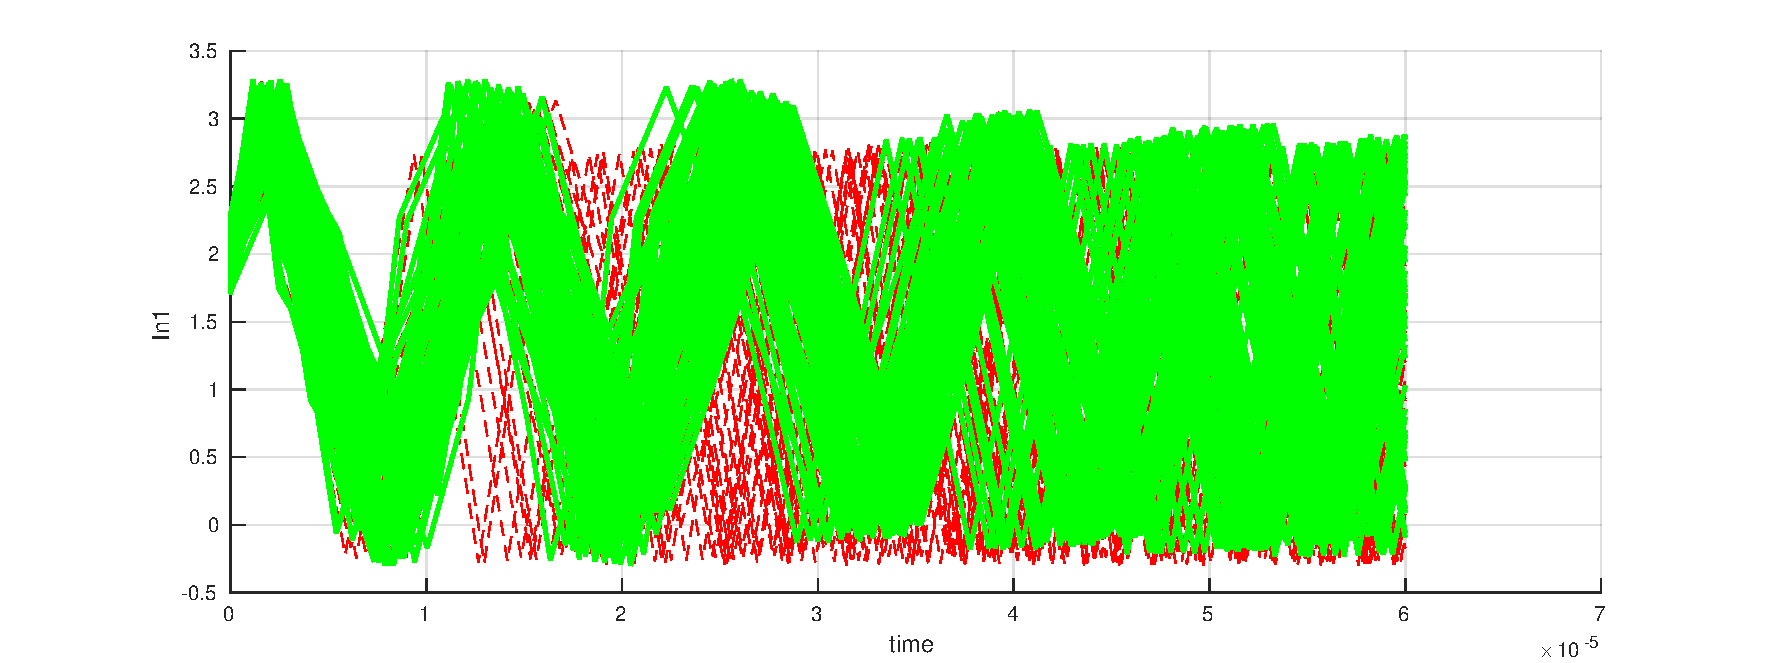
\includegraphics[width=\textwidth]{inputs_reject.png}
  \caption{The figure presents a set of $100$ signals generated with a custom method, of which 63 (green solid) satisfy the constraints of the timed automaton, and $37$ (red, dashed) do not.}
  \label{fig:reject}
 % \vspace{-3mm}
\end{figure}



%% \subsection{Benchmark experiment setup}

%% In our experiment, we try to compare the performance of a MATLAB implementation of our algorithm
%% with the following standard approaches: the uniform random sampling, CMA-ES,
%% Simulated annealing, Global Nelder Mead algorithm implementations (integrated in the same version of the tool 
%% Breach toolbox~\cite{BreachCAV10} that we used for our algorithm implementation), and the S-TaLiRo tool~\cite{TaliroLFS11} by setting Simulated Annealing as optimization algorithm\footnote{We used the latest version available in October 2016, on the site \url{https://sites.google.com/a/asu.edu/s-taliro/home}.}. Our
%% experiments were performed on a computer with 1.4GHz processor with 4GB
%% RAM, running MATLAB R2015 64-bit version. The settings of our algorithm as well as the other
%% falsification algorithm implementations are detailed below.


%% \subsubsection{Input signal specifications} 
%% \emph{Input signal range}.  We considered smaller ranges for
%% input signals than the ranges considered in the earlier
%% papers~\cite{Dreossi2015,FainekosARCH1415}, so that the properties become more robust and
%% consequently difficult to falsify.  F For the Automative Powertrain PTC example,
%% the Pedal Angle range is set as $[0,40]$ and Engine speed and Sensor
%% Offset signals are fixed as $1000$ and $1$, respectively.
%% %=======
%% %In our experiment, we try to compare the performance of our algorithm
%% %with standard approaches like uniform random sampling, CMAES,
%% %Simulated annealing, Global Nelder Mead and the an implementation
%% %distributed with the S-TaLiRo tool. Our
%% %experiments are performed on a computer with 1.4GHz processor with 4GB
%% %RAM.  The experimentes are implemented on MATLAB R2015 64-bit version.
%% %Our algorithm is implemented in the Breach toolbox~\textbf{CITE} for
%% %MATLAB-Simulink.  The setting of our algorithm as well as the other
%% %falsification algorithms is detailed below.
%% %
%% %
%% %\subsubsection{Input signal specifications} 
%% %\emph{Input signal range}.  We considered smaller ranges for input
%% %signals than the ranges considered in the earlier papers~\cite{todo},
%% %so that the properties become more robust and consequently difficult
%% %to falsify.  For the Automatic Transmission example, the throttle
%% %signal is allowed to vary between $[35,100]$ and the break is allowed
%% %to vary between $[0,40]$. For the Automative Powertrain PTC example,
%% %the Pedal Angle range is set as $[0,40]$ and Engine speed and Sensor
%% %Offset signals are fixed as $1000$ and $1$, respectively.
%% %>>>>>>> efa2003730ca38787c30f35819df6ca0f14cfe20

%% \emph{Finite parametrization of input signals.} We consider
%% piecewise constant input signals.  Furthermore, the allowed time
%% points of discontinuity for the piecewise constant signals are
%% uniformly spaced in the simulation time range of the signals.  For the
%% Automatic Transmission example, the throttle signal has $7$ control
%% points and the break signal has $3$ control points. So, we have
%% $m=7+3=10$ dimensional parameterized input signal space $\cpset$.  For the
%% Automative Powertrain Control example, we have $10$ control points,
%% thus, $\cpset$ is a $10$-dimensional space.


%% \subsubsection{Algorithm settings} 
%% \paragraph{Our algorithm setting}
%% \begin{itemize}
%% \item Threshold number of samples of hyperplane classification $K_c$ is
%% $70$ for the Automatic Transmission example and $100$ for the
%% Automative Powertrain Control example. For the Automatic Transmission
%% example, the influence of the break signal is not as much as that of the
%% throttle signal. Hence we considered a smaller threshold for
%% classification compared to the Automative Powertrain Control example.
%% %
%% \item Cell partitioning $\omega$ consists of hypercubes of side
%% length $\epsilon=4$ for both examples.
%% %
%% \item Global search time is $\Tglobalmax=500s$ for Automatic Transmission, while
%% $\Tglobalmax=2000s$ for the Automative Powertrain Control example.  The
%% Automative Powertrain example has a higher global search time because
%% the time of each function evaluation (simulation) is higher.
%% \item Local search settings. The CMA-ES implementation from
%% Breach-MATLAB toolbox was run for $4$ random number generating seeds: $0$,
%% $5000$, $10000$ and $15000$. The maximum time for the algorithm is
%% set to $2000$s for Automatic Transmission example and $5000$s for Automative Powertrain Control example.
%% \end{itemize}



%% \paragraph{S-TaLiRo setting.}  The Automatic transmission example is available in the distribution of
%% S-TaLiRo\footnote{The used distribution is available at~\url{sites.google.com/a/asu.edu/s-taliro/s-taliro/download}}.
%% For our experiment, we run the script provided in the distribution
%% with the following changes and specifications.  The range of throttle
%% input is reduced to $[35,100]$, while the original script specified
%% it as $[0,100]$.  The break input range is reduced to $[0,40]$, while
%% the original script has the range $[0,40]$.  We changed the class of
%% signals to piecewise constant.  Furthermore, we set the system to be a
%% black box, by setting the relevant S-TaLiRo options.  For the property
%% $\phi$, the script requires values for $\overline{\omega}$
%% and $\overline{v}$.  We specified them as $2520$ and $50$
%% respectively, according to the property we considered in the example.
%% The maximum number of tests (robustness evaluations) in the experiment
%% is set to $20000$.  The script runs the Simulated annealing algorithm
%% for falsification with the seed zero.  The default seed for random
%% number generation is set to $0$.


%% \paragraph{CMA-ES (in Breach) setting.}  The CMA-ES algorithm from Breach was run with the 
%% following setting.  We set the maximum time for the algorithm to $5000$s. The initialization vector is the mean of the
%% input-range.  We ran the algorithm with $4$ instances of seeds for
%% random number generation, i.e., seeds $0$, $5000$, $10000$ and $15000$.

%% \paragraph{Global-Nelder-Mead (in Breach) setting.} The
%% settings were specified in the default setup of Global-Nelder-Mead in
%% Breach.  The maximum time is set to $5000$ for the Automotive Powertrain and
%% $2000$ for the Automatic Transmission example.

%% \subsection{Benchmark results}  

%% The experimental results for the two benchmarks are reported in Table \ref{tab:results}.


%% For the Automatic Transmission example, just the global search phase
%% of our algorithm, i.e., without the CMA-ES local search, successfully
%% found a falsifier within $1000$s. In comparison, the CMA-ES algorithm
%% could not falsify within $2000$s for any of these seeds.  The uniform
%% random sampling procedure found a falsifier for only the
%% seed $15000$, but failed to find a falsifier within 2000s for the rest
%% seeds $0$, $5000$, $10000$, and $20000$.  Also, the Global Nelder Mead and
%% Simulated Annealing could not falsify within $2000$s and S-TaLiRo could
%% not falsify within $3000$s.

%% For the Automative Powertrain Control example, our algorithm successfully found
%% a falsifier within $3000$s for all the seeds.  This involved running
%% the global search phase for $2000$s followed by the CMA-ES local search
%% (until falsification).  However, the CMA-ES search alone, without
%% initialization guidance from hyperplane classification, could not
%% falsify within $5000$s for any of the above seeds.  The uniform random
%% sampling algorithm found a falsifier only for the seeds $10000$ and
%% $15000$, but failed to find falsifier within $5000$s for the rest seeds
%% $0,5000$ and $20000$.  The Global Nelder Mead and Simulated annealing
%% also could not falsify within $5000$s.


%\vspace{-1em}
%\subsection{Industrial example} 
%\input{FCexample.tex}


\bibliographystyle{abbrv}
\bibliography{bibliography} 
\end{document}
